\section{Nonhomogeneous Linear Equations}

\noindent
We'll now consider the nonhomogeneous linear second order equation
\begin{equation}
  \label{eq:5.3.1}y''+p(x)y'+q(x)y=f(x),
\end{equation}
where the forcing function $f$ isn't identically zero. The next theorem, an extension of
Theorem~\ref{thmtype:5.1.1}, gives sufficient conditions for existence and uniqueness of solutions
of initial value problems for \eqref{eq:5.3.1}. We omit the proof, which is beyond the scope of this
book.

\begin{theorem}
  \color{blue}
  \label{thmtype:5.3.1} Suppose $p$, $q$, and $f$ are continuous on an open interval $(a,b)$, let
  $x_{0}$ be any point in $(a,b)$, and let $k_{0}$ and $k_{1}$ be arbitrary real numbers. Then the
  initial value problem
  \[
    y''+p(x)y'+q(x)y=f(x),\quad y(x_{0})=k_{0},\quad y'(x_{0})=k_{1}
  \]
  has a unique solution on $(a,b)$.
\end{theorem}

To find the general solution of \eqref{eq:5.3.1} on an interval $(a,b)$ where $p$, $q$, and $f$ are
continuous, it's necessary to find the general solution of the associated homogeneous equation
\begin{equation}
  \label{eq:5.3.2}y''+p(x)y'+q(x)y=0
\end{equation}
on $(a,b)$. We call \eqref{eq:5.3.2} the {\color{blue}\it complementary equation\/} for
\eqref{eq:5.3.1}.

The next theorem shows how to find the general solution of \eqref{eq:5.3.1} if we know one solution
$y_{p}$ of \eqref{eq:5.3.1} and a fundamental set of solutions of \eqref{eq:5.3.2}. We call $y_{p}$
a {\color{blue}\it particular solution\/} of \eqref{eq:5.3.1}; it can be any solution that we can
find, one way or another.

\begin{theorem}
  \color{blue}
  \label{thmtype:5.3.2} Suppose $p$, $q$, and $f$ are continuous on $(a,b)$. Let $y_{p}$ be a
  particular solution of
  \begin{equation}
    \label{eq:5.3.3}y''+p(x)y'+q(x)y=f(x)
  \end{equation}
  on $(a,b)$, and let $\{y_{1},y_{2}\}$ be a fundamental set of solutions of the complementary
  equation
  \begin{equation}
    \label{eq:5.3.4}y''+p(x)y'+q(x)y=0
  \end{equation}
  on $(a,b)$. Then $y$ is a solution of \eqref{eq:5.3.3} on $(a,b)$ if and only if
  \begin{equation}
    \label{eq:5.3.5}y=y_{p}+c_{1}y_{1}+c_{2}y_{2},
  \end{equation}
  where $c_{1}$ and $c_{2}$ are constants.
\end{theorem}

\proof We first show that $y$ in \eqref{eq:5.3.5} is a solution of \eqref{eq:5.3.3} for any choice
of the constants $c_{1}$ and $c_{2}$. Differentiating \eqref{eq:5.3.5} twice yields
\[
  y'=y_{p}'+c_{1}y_{1}'+c_{2}y_{2}'\mbox{\quad and \quad}y''=y_{p}''+c_{1}y_{1}''+c_{2}y_{2}'',
\]
so
\begin{eqnarray*}
  y''+p(x)y'+q(x)y & = & (y_{p}''+c_{1}y_{1}''+c_{2}y_{2}'')+p(x)(y_{p}'+c_{1}y_{1}'+c_{2}y_{2}') \\
                   &   & \;+q(x)(y_{p}+c_{1}y_{1}+c_{2}y_{2})                                     \\
                   & = & (y_{p}''+p(x)y_{p}'+q(x)y_{p})+c_{1}(y_{1}''+p(x)y_{1}'+q(x)y_{1})       \\
                   &   & \;+c_{2}(y_{2}''+p(x)y_{2}'+q(x)y_{2})                                   \\
                   & = & f+c_{1}\cdot0+c_{2}\cdot0=f,
\end{eqnarray*}
since $y_{p}$ satisfies \eqref{eq:5.3.3} and $y_{1}$ and $y_{2}$ satisfy \eqref{eq:5.3.4}.

Now we'll show that every solution of \eqref{eq:5.3.3} has the form \eqref{eq:5.3.5} for some choice
of the constants $c_{1}$ and $c_{2}$. Suppose $y$ is a solution of \eqref{eq:5.3.3}. We'll show that
$y-y_{p}$ is a solution of \eqref{eq:5.3.4}, and therefore of the form
$y-y_{p}=c_{1}y_{1}+c_{2}y_{2}$, which implies \eqref{eq:5.3.5}. To see this, we compute
\begin{eqnarray*}
  (y-y_{p})''+p(x)(y-y_{p})'+q(x)(y-y_{p}) & = & (y''-y_{p}'')+p(x)(y'-y_{p}')   \\
                                           &   & +q(x)(y-y_{p})                  \\
                                           & = & (y''+p(x)y'+q(x)y)              \\
                                           &   & -(y_{p}''+p(x)y_{p}'+q(x)y_{p}) \\
                                           & = & f(x)-f(x)=0,
\end{eqnarray*}
since $y$ and $y_{p}$ both satisfy \eqref{eq:5.3.3}. \bbox

We say that \eqref{eq:5.3.5} is the {\color{blue}\it general solution of \eqref{eq:5.3.3} on
$(a,b)$.\/}

If $P_{0}$, $P_{1}$, and $F$ are continuous and $P_{0}$ has no zeros on $(a,b)$, then
Theorem~\ref{thmtype:5.3.2} implies that the general solution of
\begin{equation}
  \label{eq:5.3.6}P_{0}(x)y''+P_{1}(x)y'+P_{2}(x)y=F(x)
\end{equation}
on $(a,b)$ is $y=y_{p}+c_{1}y_{1}+c_{2}y_{2}$, where $y_{p}$ is a particular solution of
\eqref{eq:5.3.6} on $(a,b)$ and $\{y_{1},y_{2}\}$ is a fundamental set of solutions of
\[
  P_{0}(x)y''+P_{1}(x)y'+P_{2}(x)y=0
\]
on $(a,b)$. To see this, we rewrite \eqref{eq:5.3.6} as
\[
  y''+\frac{P_{1}(x)}{P_{0}(x)}y'+\frac{P_{2}(x)}{P_{0}(x)}y=\frac{F(x)}{P_{0}(x)}
\]
and apply Theorem~\ref{thmtype:5.3.2} with $p=P_{1}/P_{0}$, $q=P_{2}/P_{0}$, and $f=F/P_{0}$.

To avoid awkward wording in examples and exercises, we won't specify the interval $(a,b)$ when we
ask for the general solution of a specific linear second order equation, or for a fundamental set of
solutions of a homogeneous linear second order equation. Let's agree that this always means that we
want the general solution (or a fundamental set of solutions, as the case may be) on every open
interval on which $p$, $q$, and $f$ are continuous if the equation is of the form \eqref{eq:5.3.3},
or on which $P_{0}$, $P_{1}$, $P_{2}$, and $F$ are continuous and $P_{0}$ has no zeros, if the
equation is of the form \eqref{eq:5.3.6}. We leave it to you to identify these intervals in specific
examples and exercises.

For completeness, we point out that if $P_{0}$, $P_{1}$, $P_{2}$, and $F$ are all continuous on an
open interval $(a,b)$, but $P_{0}$ {\color{blue}\it does\/} have a zero in $(a,b)$, then
\eqref{eq:5.3.6} may fail to have a general solution on $(a,b)$ in the sense just defined.
Exercises~\ref{exer:5.1.42}--\ref{exer:5.1.44} illustrate this point for a homogeneous equation.

In this section we to limit ourselves to applications of Theorem~\ref{thmtype:5.3.2} where we can
guess at the form of the particular solution.

\begin{example}
  \label{example:5.3.1} \rm \mbox{}
  \newline
  \begin{alist}
    \item % (a)
    Find the general solution of
    \begin{equation}
      \label{eq:5.3.7}y''+y=1.
    \end{equation}

    \item % (b)
    Solve the initial value problem
    \begin{equation}
      \label{eq:5.3.8}y''+y=1,\quad y(0)=2,\quad y'(0)=7.
    \end{equation}
  \end{alist}
\end{example}

\solutionpart{a} We can apply Theorem~\ref{thmtype:5.3.2} with $(a,b)=(-\infty,\infty)$, since the
functions $p\equiv0$, $q\equiv1$, and $f\equiv1$ in \eqref{eq:5.3.7} are continuous on
$(-\infty,\infty)$. By inspection we see that $y_{p}\equiv1$ is a particular solution of
\eqref{eq:5.3.7}. Since $y_{1}=\cos x$ and $y_{2}=\sin x$ form a fundamental set of solutions of the
complementary equation $y''+y=0$, the general solution of \eqref{eq:5.3.7} is
\begin{equation}
  \label{eq:5.3.9}y=1+c_{1}\cos x+c_{2}\sin x.
\end{equation}

\solutionpart{b} Imposing the initial condition $y(0)=2$ in \eqref{eq:5.3.9} yields $2=1+c_{1}$, so
$c_{1}=1$. Differentiating \eqref{eq:5.3.9} yields
\[
  y'=-c_{1}\sin x+c_{2}\cos x.
\]
Imposing the initial condition $y'(0)=7$ here yields $c_{2}=7$, so the solution of \eqref{eq:5.3.8}
is
\[
  y=1+\cos x+7\sin x.
\]
Figure~\ref{figure:5.3.1} is a graph of this function.

\begin{figure}[tbp]
  \centering
  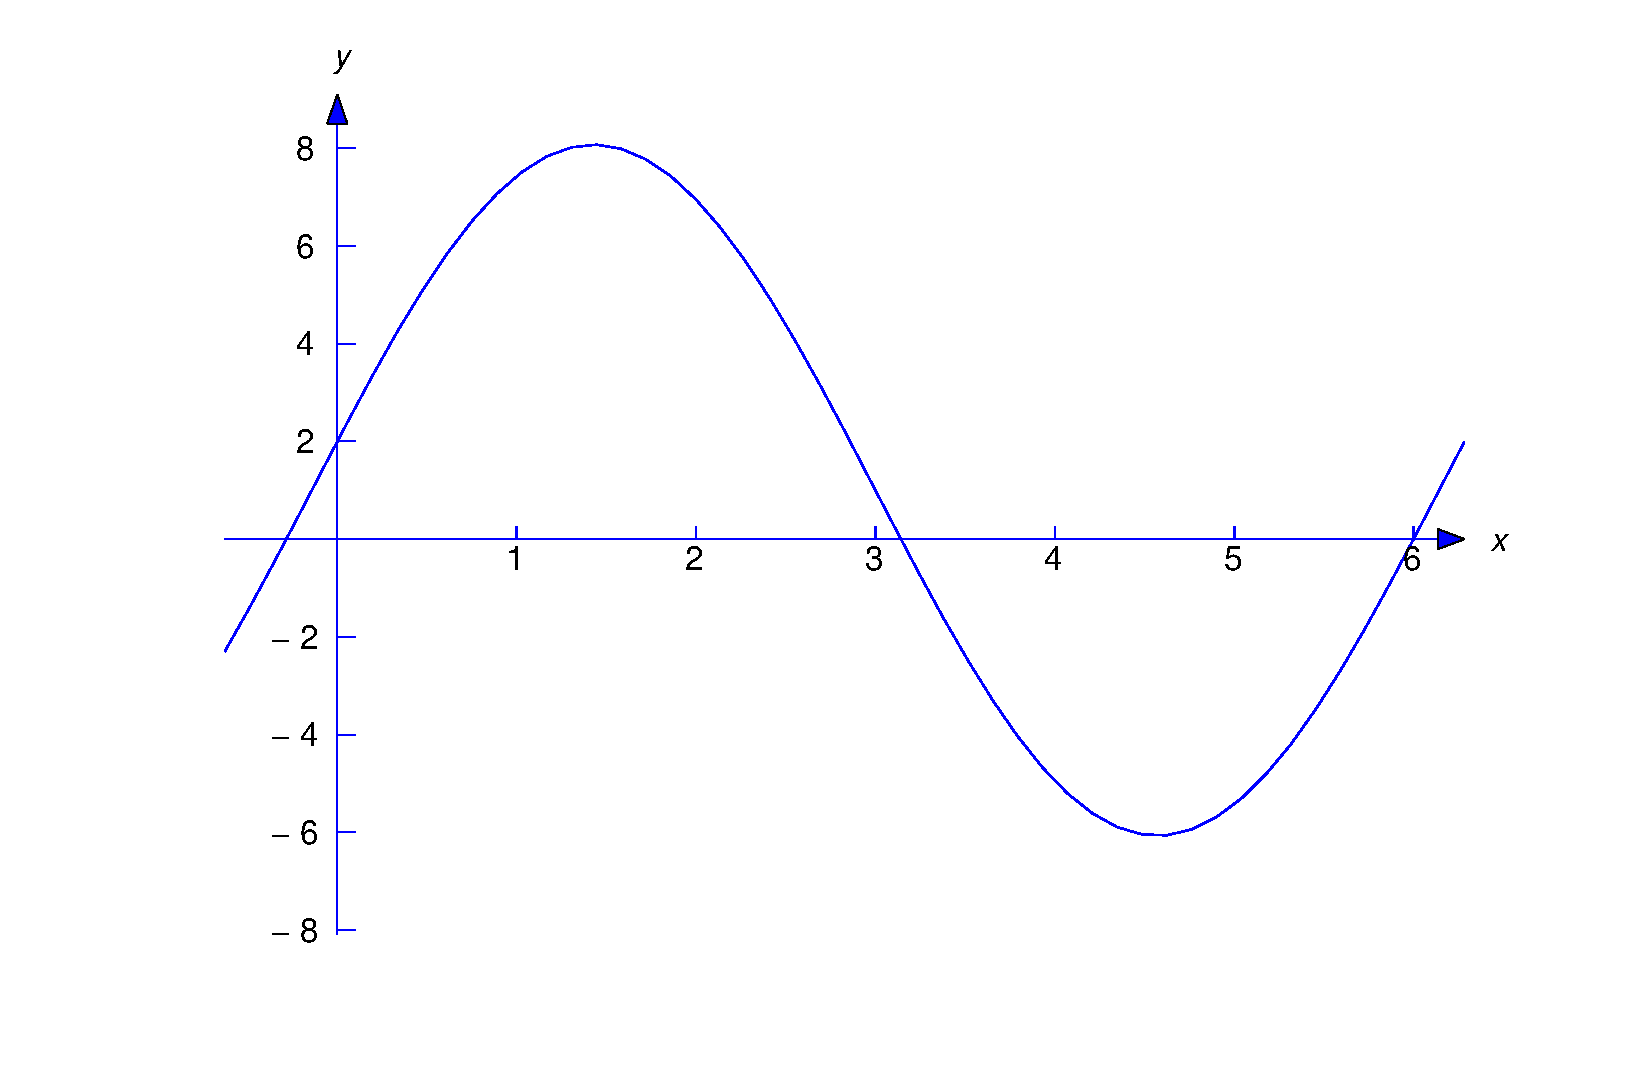
\includegraphics[bb=-78 148 689 643, width=5.67in, height=3.66in, keepaspectratio]{fig050301}
  \color{blue}
  \caption{$y=1+\cos x+7\sin x$}
  \label{figure:5.3.1}
\end{figure}

\begin{example}
  \label{example:5.3.2} \rm \mbox{}
  \newline %\examplepoly
  \begin{alist}
    \item % (a)
    Find the general solution of
    \begin{equation}
      \label{eq:5.3.10}y''-2y'+y=-3-x+x^{2}.
    \end{equation}

    \item % (b)
    Solve the initial value problem
    \begin{equation}
      \label{eq:5.3.11}y''-2y'+y=-3-x+x^{2},\quad y(0)=-2,\quad y'(0)=1.
    \end{equation}
  \end{alist}
\end{example}

\solutionpart{a} The characteristic polynomial of the complementary equation
\[
  y''-2y'+y=0
\]
is $r^{2}-2r+1=(r-1)^{2}$, so $y_{1}=e^{x}$ and $y_{2}=xe^{x}$ form a fundamental set of solutions
of the complementary equation. To guess a form for a particular solution of \eqref{eq:5.3.10}, we
note that substituting a second degree polynomial $y_{p}=A+Bx+Cx^{2}$ into the left side of
\eqref{eq:5.3.10} will produce another second degree polynomial with coefficients that depend upon
$A$, $B$, and $C$. The trick is to choose $A$, $B$, and $C$ so the polynomials on the two sides of
\eqref{eq:5.3.10} have the same coefficients; thus, if
\[
  y_{p}=A+Bx+Cx^{2}\mbox{\quad then \quad}y_{p}'=B+2Cx\mbox{\quad and \quad}y_{p}''=2C,
\]
so
\begin{eqnarray*}
  y_{p}''-2y_{p}'+y_{p} & = & 2C-2(B+2Cx)+(A+Bx+Cx^{2}) \\
                        & = & (2C-2B+A)+(-4C+B)x+Cx^{2}=-3-x+x^{2}.
\end{eqnarray*}
Equating coefficients of like powers of $x$ on the two sides of the last equality yields
\begin{eqnarray*}
  C       & = & \phantom{-}1\phantom{.} \\
  B-4C    & = & -1\phantom{.}           \\
  A-2B+2C & = & -3,
\end{eqnarray*}
so $C=1$, $B=-1+4C=3$, and $A=-3-2C+2B=1$. Therefore $y_{p}=1+3x+x^{2}$ is a particular solution of
\eqref{eq:5.3.10} and Theorem~\ref{thmtype:5.3.2} implies that
\begin{equation}
  \label{eq:5.3.12}y=1+3x+x^{2}+e^{x}(c_{1}+c_{2}x)
\end{equation}
is the general solution of \eqref{eq:5.3.10}.

\solutionpart{b} Imposing the initial condition $y(0)=-2$ in \eqref{eq:5.3.12} yields $-2=1+c_{1}$,
so $c_{1}=-3$. Differentiating \eqref{eq:5.3.12} yields
\[
  y'=3+2x+e^{x}(c_{1}+c_{2}x)+c_{2}e^{x},
\]
and imposing the initial condition $y'(0)=1$ here yields $1=3+c_{1}+c_{2}$, so $c_{2}=1$. Therefore
the solution of \eqref{eq:5.3.11} is
\[
  y=1+3x+x^{2}-e^{x}(3-x).
\]
Figure~\ref{figure:5.3.2} is a graph of this solution.

\begin{figure}[tbp]
  \centering
  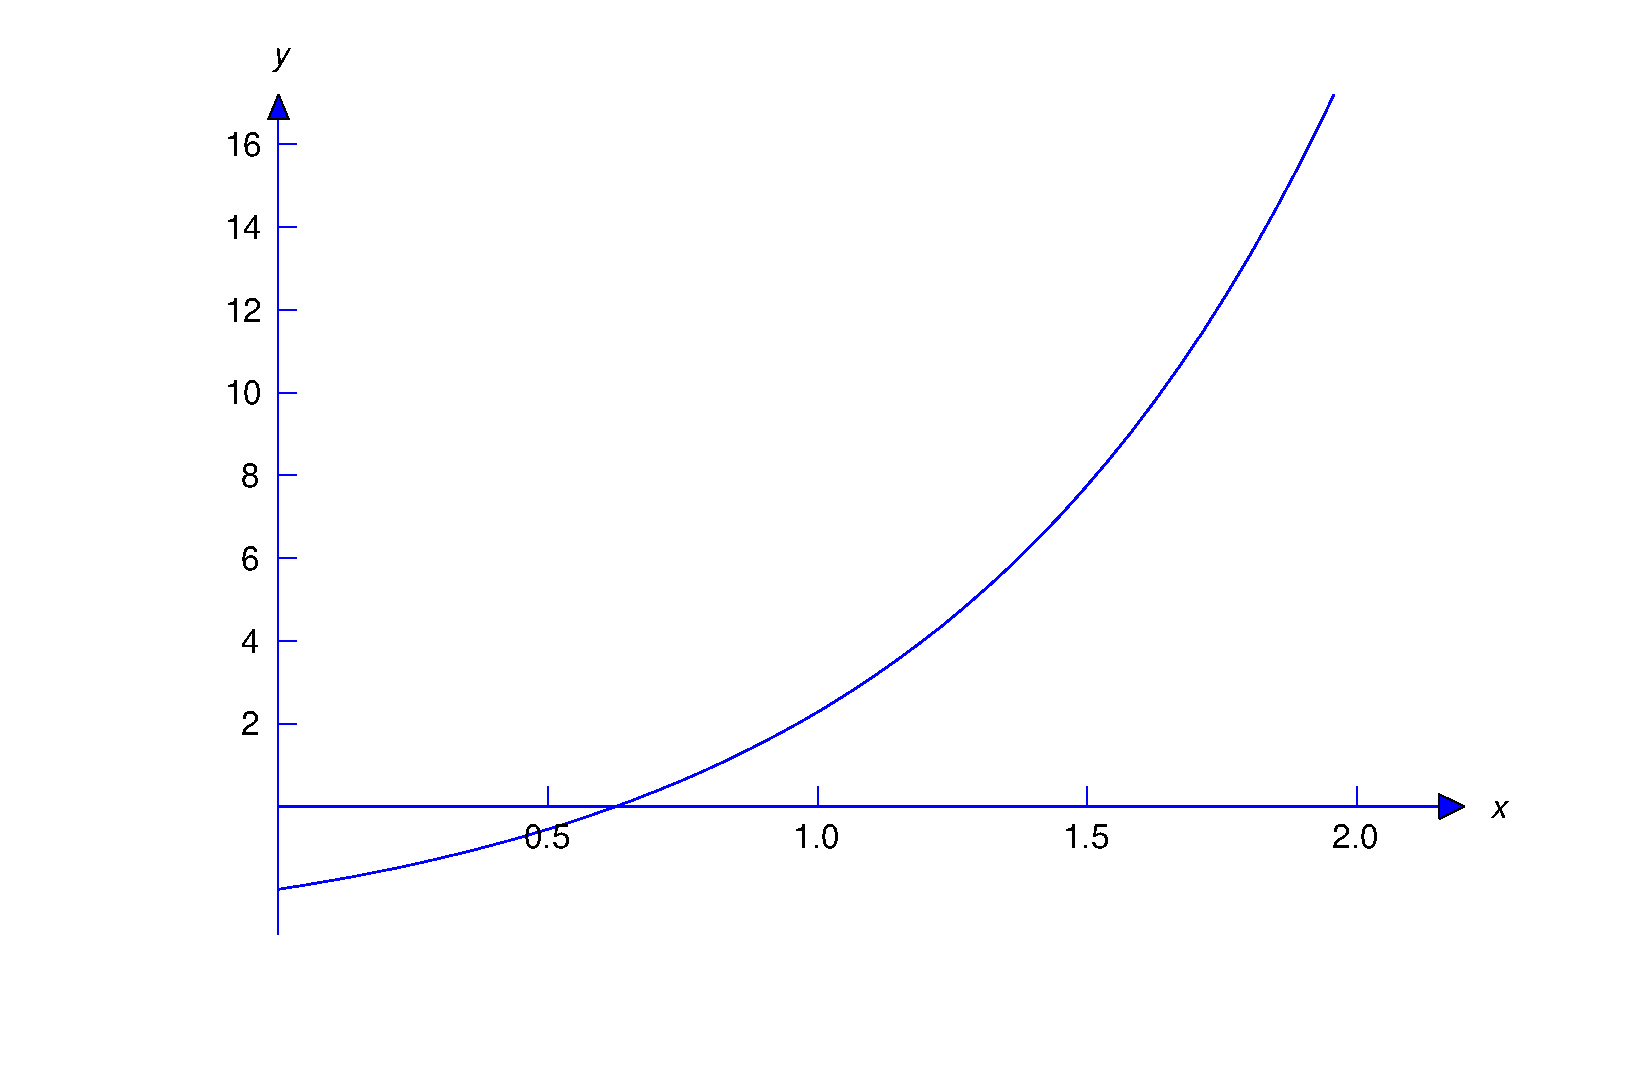
\includegraphics[bb=-78 148 689 643, width=5.67in, height=3.66in, keepaspectratio]{fig050302}
  \color{blue}
  \caption{$y=1+3x+x^{2}-e^{x}(3-x)$}
  \label{figure:5.3.2}
\end{figure}

\begin{example}
  \label{example:5.3.3} \rm Find the general solution of
  \begin{equation}
    \label{eq:5.3.13}x^{2}y''+xy'-4y=2x^{4}
  \end{equation}
  on $(-\infty,0)$ and $(0,\infty)$.
\end{example}

\solution In Example~\ref{example:5.1.3}, we verified that $y_{1}=x^{2}$ and $y_{2}=1/x^{2}$ form a
fundamental set of solutions of the complementary equation
\[
  x^{2}y''+xy'-4y=0
\]
on $(-\infty,0)$ and $(0,\infty)$. To find a particular solution of \eqref{eq:5.3.13}, we note that
if $y_{p}=Ax^{4}$, where $A$ is a constant then both sides of \eqref{eq:5.3.13} will be constant
multiples of $x^{4}$ and we may be able to choose $A$ so the two sides are equal. This is true in
this example, since if $y_{p}=Ax^{4}$ then
\[
  x^{2}y_{p}''+xy_{p}'-4y_{p}=x^{2}(12Ax^{2})+x(4Ax^{3})-4Ax^{4}=12Ax^{4}=2x^{4}
\]
if $A=1/6$; therefore, $y_{p}=x^{4}/6$ is a particular solution of \eqref{eq:5.3.13} on
$(-\infty,\infty)$. Theorem~\ref{thmtype:5.3.2} implies that the general solution of
\eqref{eq:5.3.13} on $(-\infty,0)$ and $(0,\infty)$ is
\[
  y=\frac{x^{4}}{6}+c_{1}x^{2}+\frac{c_{2}}{x^{2}}.
\]

\boxit{The Principle of Superposition}

\noindent
The next theorem enables us to break a nonhomogeneous equation into simpler parts, find a particular
solution for each part, and then combine their solutions to obtain a particular solution of the
original problem.

\begin{theorem}
  \color{blue}
  $[$The Principle of Superposition$]$ \label{thmtype:5.3.3} Suppose $y_{p_{1}}$ is a particular
  solution of
  \[
    y''+p(x)y'+q(x)y=f_{1}(x)
  \]
  on $(a,b)$ and $y_{p_{2}}$ is a particular solution of
  \[
    y''+p(x)y'+q(x)y=f_{2}(x)
  \]
  on $(a,b)$. Then
  \[
    y_{p}=y_{p_{1}}+y_{p_{2}}
  \]
  is a particular solution of
  \[
    y''+p(x)y'+q(x)y=f_{1}(x)+f_{2}(x)
  \]
  on $(a,b)$.
\end{theorem}

\proof If $y_{p}=y_{p_{1}}+y_{p_{2}}$ then
\begin{eqnarray*}
  y_{p}''+p(x)y_{p}'+q(x)y_{p} & = & (y_{p_{1}}+y_{p_{2}})''+p(x)(y_{p_{1}}+y_{p_{2}})'+q(x)(y_{p_{1}}+y_{p_{2}})                                \\
                               & = & \left(y_{p_{1}}''+p(x)y_{p_{1}}'+q(x)y_{p_{1}}\right)+\left(y_{p_{2}}''+p(x)y_{p_{2}}'+q(x)y_{p_{2}}\right) \\
                               & = & f_{1}(x)+f_{2}(x).\bbox
\end{eqnarray*}

It's easy to generalize Theorem~\ref{thmtype:5.3.3} to the equation
\begin{equation}
  \label{eq:5.3.14}y''+p(x)y'+q(x)y=f(x)
\end{equation}
where
\[
  f=f_{1}+f_{2}+\cdots+f_{k};
\]
thus, if $y_{p_{i}}$ is a particular solution of
\[
  y''+p(x)y'+q(x)y=f_{i}(x)
\]
on $(a,b)$ for $i=1$, $2$, \dots, $k$, then $y_{p_{1}}+y_{p_{2}}+\cdots+y_{p_{k}}$ is a particular
solution of \eqref{eq:5.3.14} on $(a,b)$. Moreover, by a proof similar to the proof of
Theorem~\ref{thmtype:5.3.3} we can formulate the principle of superposition in terms of a linear
equation written in the form
\[
  P_{0}(x)y''+P_{1}(x)y'+P_{2}(x)y=F(x)
\]
(Exercise~\ref{exer:5.3.39}); that is, if $y_{p_{1}}$ is a particular solution of
\[
  P_{0}(x)y''+P_{1}(x)y'+P_{2}(x)y=F_{1}(x)
\]
on $(a,b)$ and $y_{p_{2}}$ is a particular solution of
\[
  P_{0}(x)y''+P_{1}(x)y'+P_{2}(x)y=F_{2}(x)
\]
on $(a,b)$, then $y_{p_{1}}+y_{p_{2}}$ is a solution of
\[
  P_{0}(x)y''+P_{1}(x)y'+P_{2}(x)y=F_{1}(x)+F_{2}(x)
\]
on $(a,b)$.

\begin{example}
  \label{example:5.3.4} \rm The function $y_{p_{1}}=x^{4}/15$ is a particular solution of
  \begin{equation}
    \label{eq:5.3.15}x^{2}y''+4xy'+2y=2x^{4}
  \end{equation}
  on $(-\infty,\infty)$ and $y_{p_{2}}=x^{2}/3$ is a particular solution of
  \begin{equation}
    \label{eq:5.3.16}x^{2}y''+4xy'+2y=4x^{2}
  \end{equation}
  on $(-\infty,\infty)$. Use the principle of superposition to find a particular solution of
  \begin{equation}
    \label{eq:5.3.17}x^{2}y''+4xy'+2y=2x^{4}+4x^{2}
  \end{equation}
  on $(-\infty,\infty)$.
\end{example}

\solution The right side $F(x)=2x^{4}+4x^{2}$ in \eqref{eq:5.3.17} is the sum of the right sides
\[
  F_{1}(x)=2x^{4}\quad\mbox{ and }\quad F_{2}(x)=4x^{2}.
\]
in \eqref{eq:5.3.15} and \eqref{eq:5.3.16}. Therefore the principle of superposition implies that
\[
  y_{p}=y_{p_{1}}+y_{p_{2}}=\frac{x^{4}}{15}+\frac{x^{2}}{3}
\]
is a particular solution of \eqref{eq:5.3.17}.

\exercises

\noindent
In Exercises~\ref{exer:5.3.1}--\ref{exer:5.3.6} find a particular solution by the method used in
Example~\ref{example:5.3.2}. Then find the general solution and, where indicated, solve the initial
value problem and graph the solution.

\begin{exerciselist}
  \item\label{exer:5.3.1} $y''+5y'-6y=22+18x-18x^{2}$

  \item\label{exer:5.3.2} $y''-4y'+5y=1+5x$

  \item\label{exer:5.3.3} $y''+8y'+7y=-8-x+24x^{2}+7x^{3}$

  \item\label{exer:5.3.4} $y''-4y'+4y=2+8x-4x^{2}$

  \item\label{exer:5.3.5} \CGex $y''+2y'+10y=4+26x+6x^{2}+10x^{3},\quad y(0)=2, \quad y'(0)=9$

  \item\label{exer:5.3.6} \CGex $y''+6y'+10y=22+20x,\quad y(0)=2,\; y'(0)=-2$

  \item\label{exer:5.3.7} Show that the method used in Example~\ref{example:5.3.2} won't yield a
        particular solution of
  \[
    y''+y'=1+2x+x^{2}; \eqno{\rm(A)}
  \]
  that is, (A) doesn't have a particular solution of the form $y_{p}=A+Bx+Cx^{2}$, where $A$, $B$,
  and $C$ are constants.

  \exercisetext{In Exercises~\ref{exer:5.3.8}--\ref{exer:5.3.13} find a particular solution by the
  method used in Example~\ref{example:5.3.3}.}

  \begin{tabular}[t]{@{}p{168pt}@{}p{168pt}}
    \item\label{exer:5.3.8} $x^{2}y''+7xy'+8y=\dst\frac{6}{x}$ &
    \item\label{exer:5.3.9} $x^{2}y''-7xy'+7y=13x^{1/2}$
  \end{tabular}

  \begin{tabular}[t]{@{}p{168pt}@{}p{168pt}}
    \item\label{exer:5.3.10} $x^{2}y''-xy'+y=2x^{3}$ &
    \item\label{exer:5.3.11} $x^{2}y''+5xy'+4y=\dst\frac{1}{x^{3}}$
  \end{tabular}

  \begin{tabular}[t]{@{}p{168pt}@{}p{168pt}}
    \item\label{exer:5.3.12} $x^{2}y''+xy'+y=10x^{1/3}$ &
    \item\label{exer:5.3.13} $x^{2}y''-3xy'+13y=2x^{4}$
  \end{tabular}

  \item\label{exer:5.3.14} Show that the method suggested for finding a particular solution in
        Exercises~\ref{exer:5.3.8}-\ref{exer:5.3.13} won't yield a particular solution of
  \[
    x^{2}y''+3xy'-3y=\frac{1}{x^{3}}; \eqno{\rm(A)}
  \]
  that is, (A) doesn't have a particular solution of the form $y_{p}=A/x^{3}$.

  \item\label{exer:5.3.15} Prove: If $a$, $b$, $c$, $\alpha$, and $M$ are constants and $M\ne0$ then
  \[
    ax^{2}y''+bxy'+cy=Mx^{\alpha}
  \]
  has a particular solution $y_{p}=Ax^{\alpha}$ ($A=$ constant) if and only if
  $a\alpha(\alpha-1)+b\alpha+c\ne0$.

  \exercisetext{If $a$, $b$, $c$, and $\alpha$ are constants, then \[a(e^{\alpha x})''+b(e^{\alpha
  x})'+ce^{\alpha x}=(a\alpha^{2}+b\alpha+c)e^{\alpha x}.\] Use this in
  Exercises~\ref{exer:5.3.16}--\ref{exer:5.3.21} to find a particular solution . Then find the
  general solution and, where indicated, solve the initial value problem and graph the solution.}
  %Exercises~\ref{exer:5.3.16}--\ref{exer:5.3.21} are referenced later as
  %\exercisec.

  \begin{tabular}[t]{@{}p{168pt}@{}p{168pt}}
    \item\label{exer:5.3.16} $y''+5y'-6y=6e^{3x}$ & \vspace*{10pt}
    \item\label{exer:5.3.17} $y''-4y'+5y=e^{2x}$
  \end{tabular}

  \item\label{exer:5.3.18} \CGex $y''+8y'+7y=10e^{-2x},\quad y(0)=-2,\; y'(0)=10$

  \item\label{exer:5.3.19} \CGex $y''-4y'+4y=e^{x},\quad y(0)=2,\quad y'(0)=0$

  \begin{tabular}[t]{@{}p{168pt}@{}p{168pt}}
    \item\label{exer:5.3.20} $y''+2y'+10y=e^{x/2}$ &
    \item\label{exer:5.3.21} $y''+6y'+10y=e^{-3x}$
  \end{tabular}

  \item\label{exer:5.3.22} Show that the method suggested for finding a particular solution in
        Exercises~\ref{exer:5.3.16}-\ref{exer:5.3.21} won't yield a particular solution of
  \[
    y''-7y'+12y=5e^{4x}; \eqno{\rm(A)}
  \]
  that is, (A) doesn't have a particular solution of the form $y_{p}=Ae^{4x}$.

  \item\label{exer:5.3.23} Prove: If $\alpha$ and $M$ are constants and $M\ne0$ then constant
        coefficient equation
  \[
    ay''+by'+cy=Me^{\alpha x}
  \]
  has a particular solution $y_{p}=Ae^{\alpha x}$ ($A=$ constant) if and only if $e^{\alpha x}$
  isn't a solution of the complementary equation.

  \exercisetext{If $\omega$ is a constant, differentiating a linear combination of $\cos\omega x$
  and $\sin\omega x$ with respect to $x$ yields another linear combination of $\cos\omega x$ and
  $\sin\omega x$. In Exercises~\ref{exer:5.3.24}--\ref{exer:5.3.29} use this to find a particular
  solution of the equation. Then find the general solution and, where indicated, solve the initial
  value problem and graph the solution.}

  \item\label{exer:5.3.24} $y''-8y'+16y=23\cos x-7\sin x$

  \item\label{exer:5.3.25} $y''+y'=-8\cos2x+6\sin2x$

  \item\label{exer:5.3.26} $y''-2y'+3y=-6\cos3x+6\sin3x$

  \item\label{exer:5.3.27}$y''+6y'+13y=18\cos x+6\sin x$

  \item\label{exer:5.3.28} \CGex $y''+7y'+12y=-2\cos2x+36\sin2x,\quad y(0)=-3,\quad y'(0)=3$

  \item\label{exer:5.3.29} \CGex $y''-6y'+9y=18\cos3x+18\sin3x,\quad y(0)=2,\quad y'(0)=2$

  \item\label{exer:5.3.30} Find the general solution of
  \[
    y''+\omega_{0}^{2}y=M\cos\omega x+N\sin\omega x,
  \]
  where $M$ and $N$ are constants and $\omega$ and $\omega_{0}$ are distinct positive numbers.

  \item\label{exer:5.3.31} Show that the method suggested for finding a particular solution in
        Exercises~\ref{exer:5.3.24}-\ref{exer:5.3.29} won't yield a particular solution of
  \[
    y''+y=\cos x+\sin x; \eqno{\rm(A)}
  \]
  that is, (A) does not have a particular solution of the form $y_{p}=A\cos x+B\sin x$.

  \item\label{exer:5.3.32} Prove: If $M$, $N$ are constants (not both zero) and $\omega>0$, the
        constant coefficient equation
  \[
    ay''+by'+cy=M\cos\omega x+N\sin\omega x \eqno{\rm(A)}
  \]
  has a particular solution that's a linear combination of $\cos\omega x$ and $\sin\omega x$ if and
  only if the left side of (A) is not of the form $a(y''+\omega^{2}y)$, so that $\cos\omega x$ and
  $\sin\omega x$ are solutions of the complementary equation.

  \exercisetext{In Exercises~\ref{exer:5.3.33}--\ref{exer:5.3.38} refer to the cited exercises and
  use the principal of superposition to find a particular solution. Then find the general solution.}

  \item\label{exer:5.3.33} $y''+5y'-6y=22+18x-18x^{2}+6e^{3x}$ (See Exercises~\ref{exer:5.3.1} and
        \ref{exer:5.3.16}.)

  \item\label{exer:5.3.34} $y''-4y'+5y=1+5x+e^{2x}$ (See Exercises~\ref{exer:5.3.2} and
        \ref{exer:5.3.17}.)

  \item\label{exer:5.3.35} $y''+8y'+7y=-8-x+24x^{2}+7x^{3}+10e^{-2x}$ (See
        Exercises~\ref{exer:5.3.3} and \ref{exer:5.3.18}.)

  \item\label{exer:5.3.36} $y''-4y'+4y=2+8x-4x^{2}+e^{x}$ (See Exercises~\ref{exer:5.3.4} and
        \ref{exer:5.3.19}.)

  \item\label{exer:5.3.37} $y''+2y'+10y=4+26x+6x^{2}+10x^{3}+e^{x/2}$ (See
        Exercises~\ref{exer:5.3.5} and \ref{exer:5.3.20}.)

  \item\label{exer:5.3.38} $y''+6y'+10y=22+20x+e^{-3x}$ (See Exercises~\ref{exer:5.3.6} and
        \ref{exer:5.3.21}.)

  \item\label{exer:5.3.39} Prove: If $y_{p_{1}}$ is a particular solution of
  \[
    P_{0}(x)y''+P_{1}(x)y'+P_{2}(x)y=F_{1}(x)
  \]
  on $(a,b)$ and $y_{p_{2}}$ is a particular solution of
  \[
    P_{0}(x)y''+P_{1}(x)y'+P_{2}(x)y=F_{2}(x)
  \]
  on $(a,b)$, then $y_{p}=y_{p_{1}}+y_{p_{2}}$ is a solution of
  \[
    P_{0}(x)y''+P_{1}(x)y'+P_{2}(x)y=F_{1}(x)+F_{2}(x)
  \]
  on $(a,b)$.

  \item\label{exer:5.3.40} Suppose $p$, $q$, and $f$ are continuous on $(a,b)$. Let $y_{1}$,
        $y_{2}$, and $y_{p}$ be twice differentiable on $(a,b)$, such that
        $y=c_{1}y_{1}+c_{2}y_{2}+y_{p}$ is a solution of
  \[
    y''+p(x)y'+q(x)y=f
  \]
  on $(a,b)$ for every choice of the constants $c_{1}$, $c_{2}$. Show that $y_{1}$ and $y_{2}$ are
  solutions of the complementary equation on $(a,b)$.
\end{exerciselist}
